% ulm-lam-howto.tex -- How to build ulm.lam, step by step.
% Build: latexmk (LuaLaTeX, see latexmkrc).  The listings in outputs/ are
% produced by examples/run.sh.
\documentclass[11pt,a4paper]{article}

\usepackage{fontspec}
\usepackage{unicode-math}
\setmainfont{Libertinus Serif}
\setsansfont{Libertinus Sans}
\setmathfont{Libertinus Math}
\setmonofont{JuliaMono}[Scale=MatchLowercase]

\usepackage[margin=2.5cm]{geometry}
\usepackage{microtype}
\usepackage{booktabs,tabularx,array}
\usepackage[inline]{enumitem}
\usepackage[skip=\medskipamount]{parskip}
\usepackage{xcolor,luacolor,lua-ul}
\usepackage{listings}
\usepackage{xparse}
\usepackage{tikz}
\usetikzlibrary{positioning,arrows.meta}
\usepackage[hidelinks]{hyperref}
\usepackage[nameinlink,capitalise,noabbrev]{cleveref}
\crefname{section}{Step}{Steps}
\Crefname{section}{Step}{Steps}
\crefname{appendix}{Appendix}{Appendices}

\setlist{itemsep=2pt,topsep=4pt}
\renewcommand{\arraystretch}{1.15}
\renewcommand{\thesection}{\arabic{section}}
% sections are the steps: "Step 3  The operations of linear algebra"
\makeatletter
\newcommand{\presection}{Step~}
\renewcommand{\@seccntformat}[1]{\csname pre#1\endcsname\csname the#1\endcsname\quad}
\makeatother
\setlength{\emergencystretch}{3em}

% ---------------------------------------------------------------- notation
\newcommand{\T}{^{\mkern-1.5mu\mathsf{T}}}
\newcommand{\inv}{^{-1}}
\newcommand{\invT}{^{-\mathsf{T}}}

% ---------------------------------------------------------------- colours
\definecolor{kw}{HTML}{1F4E9A}
\definecolor{cm}{HTML}{6B6B6B}
\definecolor{st}{HTML}{8A3B12}
\definecolor{ty}{HTML}{2E6B30}
\definecolor{bg}{gray}{0.95}      % code blocks
\definecolor{ttbg}{gray}{0.92}    % inline typewriter text
\definecolor{written}{HTML}{8A3B12}
\definecolor{generated}{HTML}{1F4E9A}
\definecolor{provided}{HTML}{2E6B30}

% Grey background behind \texttt via lua-ul leaders: no effect on line
% spacing, line breaks still possible.
\let\origtexttt\texttt
\renewcommand{\texttt}[1]{\highLight[ttbg]{\origtexttt{#1}}}
% inline code, verbatim argument (not inside other arguments)
\NewDocumentCommand{\code}{v}{\texttt{#1}}

% ---------------------------------------------------------------- listings
\lstdefinelanguage{mlir}{
  alsoletter={.,_,\%,\#,!,@},
  morekeywords={func.func,return,func.call,module},
  morekeywords=[2]{ulm_lam.mul,ulm_lam.add,ulm_lam.scale,ulm_lam.transpose,
    ulm_lam.inverse,ulm_lam.identity,ulm_lam.assume,ulm_lamk.gemm,
    ulm_lamk.syrk,ulm_lamk.gemv,ulm_lamk.trsv,ulm_lamk.trsm,ulm_lamk.potrf},
  morekeywords=[3]{tensor,memref,f64,i64,i8,index},
  morecomment=[l]{//},
  morestring=[b]",
  sensitive=true}
\lstdefinelanguage{tablegen}{
  morekeywords={def,class,let,include,dag,string,list,code,bit,int},
  morekeywords=[2]{ins,outs},
  morecomment=[l]{//},
  morestring=[b]",
  sensitive=true}
\lstdefinestyle{base}{
  basicstyle=\ttfamily\footnotesize,
  keywordstyle=\color{kw}\bfseries,
  keywordstyle=[2]\color{kw},
  keywordstyle=[3]\color{ty},
  commentstyle=\color{cm}\itshape,
  stringstyle=\color{st},
  backgroundcolor=\color{bg},
  frame=none,
  xleftmargin=4pt, xrightmargin=4pt,
  framexleftmargin=4pt, framexrightmargin=4pt,
  aboveskip=4pt, belowskip=8pt,
  columns=fullflexible, keepspaces=true,
  showstringspaces=false, breaklines=true,
  postbreak=\mbox{\textcolor{cm}{$\hookrightarrow$}\space},
  upquote=true, tabsize=8}
\lstdefinestyle{mlir}{style=base,language=mlir}
\lstdefinestyle{td}{style=base,language=tablegen}
\lstdefinestyle{cpp}{style=base,language=C++,
  morekeywords={override,constexpr,nullptr}}
\lstdefinestyle{py}{style=base,language=Python}
\lstdefinestyle{sh}{style=base,language=bash}
\lstdefinestyle{out}{style=base}

% Who wrote a listing: by hand, mlir-tblgen, or MLIR itself.
\newcommand{\origin}[3]{%
  \par\noindent{\raggedright\sffamily\small\textcolor{#1}{\rule[0.1ex]{0.8ex}{0.8ex}}%
  \enspace\textbf{\textcolor{#1}{#2}}\enspace #3\par}\nopagebreak[4]}
\newcommand{\written}[1]{\origin{written}{Written by hand:}{#1}}
\newcommand{\generated}[1]{\origin{generated}{Generated:}{#1}}
\newcommand{\provided}[1]{\origin{provided}{Provided by MLIR:}{#1}}
\newcommand{\shown}[1]{\origin{cm}{Output:}{#1}}

% A box at the start of every step: the mathematics, before any code.
\newenvironment{maths}{\par\medskip\noindent\begin{minipage}{\linewidth}%
  \setlength{\parskip}{\medskipamount}\sffamily\small
  \textbf{The mathematics.}\enspace}{\end{minipage}\par\medskip}

\title{How to Build ulm.lam (Ulm Linear Algebra Mapping)\\[0.3ex]
  \large A compiler for linear algebra with MLIR (Multi-Level Intermediate
  Representation), step by step}
\author{Michael Lehn}
\date{November 2026}

\begin{document}
\maketitle

\begin{abstract}
\noindent
ulm.lam turns a formula such as
\(b=(X\T M\inv X)\inv X\T M\inv y\) into a sequence of calls of BLAS
(Basic Linear Algebra Subprograms) and LAPACK (Linear Algebra PACKage)
routines, the code an expert would write by hand: it solves the LAMP
(Linear Algebra Mapping Problem). It is built on MLIR~\cite{mlir}, a framework for
writing compilers, and its central data structure is an IR (intermediate
representation) of the program. This document describes, step by step, what has to be done to
build such a compiler: which rules from linear algebra are needed, how each
of them is written down for MLIR, and which parts of the code are written by
hand, which are generated from short declarations, and which MLIR provides
ready to use. Every step starts with the mathematics, so that it can be
followed without knowing MLIR. All program output shown is produced by a
script in the repository (\cref{app:repro}).
\end{abstract}

\tableofcontents

% =====================================================================
\section*{What we build}
\addcontentsline{toc}{section}{What we build}
\label{sec:intro}

The LAMP is the task of computing a
linear algebra expression with the kernels of a library such as BLAS and
LAPACK, as efficiently as possible~\cite{lamp}. Psarras, Barthels and
Bientinesi showed that the popular high-level languages (Julia, MATLAB
(Matrix Laboratory), Octave, NumPy (Numerical Python), Armadillo, Eigen,
R) solve
this problem poorly: they evaluate formulas as written, form inverses
explicitly, ignore matrix properties, and repeat work that could be shared.
Their paper is organised by twelve experiments, one per ability a solution
of the LAMP needs. This document is its practical counterpart: it shows,
step by step, how a compiler acquires these abilities.

Our running example is GLS (generalised least squares):
\[
  b \;=\; (X\T M\inv X)\inv X\T M\inv y
\]
with \(X\in\mathbb{R}^{2000\times200}\) of full rank,
\(M\in\mathbb{R}^{2000\times2000}\) symmetric positive definite, and
\(y\in\mathbb{R}^{2000}\).
Written as is, this costs two inverses and five products. An expert writes
instead:
\begin{enumerate}
\item factorise \(M=LL\T\) (Cholesky),
\item \(W=L\inv X\) (one triangular solve with 200 right-hand sides),
\item \(S=W\T W\) (only one triangle, half the work of a general product),
\item factorise \(S=RR\T\) (Cholesky again),
\item \(z=L\inv y\), \(t=W\T z\), and \(b=R\invT R\inv t\) (four
  operations on vectors).
\end{enumerate}
No inverse is formed, \(M\) is factorised once although it is inverted
twice, and \(L\inv X\) is computed once and used twice. ulm.lam derives
exactly this sequence. At the end of this document, the generated C++ code
makes eight calls of library routines.

\subsection*{The plan}

A compiler is a chain of translations. ulm.lam has the following ones; each
section of this document adds one link of the chain.

\begin{center}
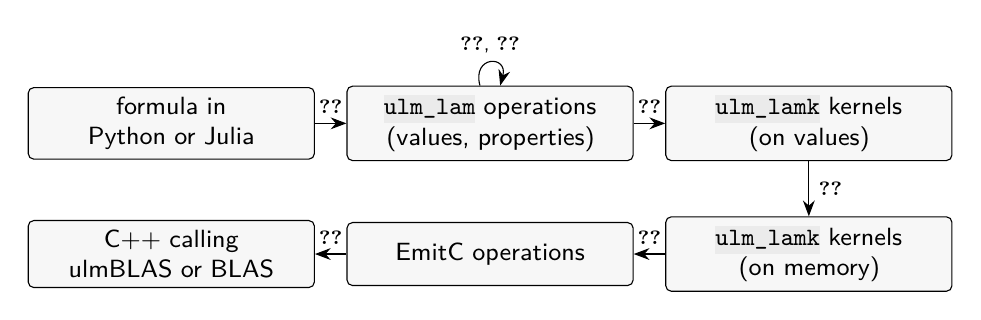
\begin{tikzpicture}[font=\sffamily\small, node distance=4mm,
  box/.style={draw, rounded corners=2pt, align=center, minimum height=8mm,
    text width=34mm, fill=black!3},
  arr/.style={-{Stealth[length=2mm]}}]
\node[box] (f) {formula in Python or Julia};
\node[box, right=of f] (l) {\texttt{ulm\_lam} operations\\(values, properties)};
\node[box, right=of l] (k) {\texttt{ulm\_lamk} kernels\\(on values)};
\node[box, below=7mm of k] (b) {\texttt{ulm\_lamk} kernels\\(on memory)};
\node[box, left=of b] (e) {EmitC operations};
\node[box, left=of e] (c) {C++ calling\\ulmBLAS or BLAS};
\draw[arr] (f) -- node[above, font=\sffamily\scriptsize] {\ref{sec:build}} (l);
\draw[arr] (l) -- node[above, font=\sffamily\scriptsize] {\ref{sec:select}} (k);
\draw[arr] (k) -- node[right, font=\sffamily\scriptsize] {\ref{sec:memory}} (b);
\draw[arr] (b) -- node[above, font=\sffamily\scriptsize] {\ref{sec:lower}} (e);
\draw[arr] (e) -- node[above, font=\sffamily\scriptsize] {\ref{sec:lower}} (c);
\draw[arr, loop above, looseness=4] (l) to node[above, font=\sffamily\scriptsize]
  {\ref{sec:rules}, \ref{sec:infer}} (l);
\end{tikzpicture}
\end{center}

The numbers on the arrows are the steps; these are:
\begin{enumerate}
\item Programs as values: what an IR is.
\item Matrix properties as part of a type.
\item The operations of linear algebra.
\item Building the IR: from a parser or from a frontend.
\item Rewrite rules: a normal form.
\item Inferring properties.
\item Kernels as operations.
\item Kernel selection: solving the LAMP.
\item From values to memory.
\item LAPACK conventions: workspace and error codes.
\item Lowering to C++.
\item Assembling the compiler, and testing it.
\end{enumerate}

\subsection*{Three kinds of code}

The question that runs through every step is: \emph{what do we have to
write, and what do we get?} Code in an MLIR project comes from three
sources, and every listing in this document is marked with its source:

\written{the code we write: declarations in TableGen and C++ (and the
frontends in Python and Julia).}
\generated{C++ that \texttt{mlir-tblgen} produces from our TableGen
declarations when the compiler is built.}
\provided{the libraries of MLIR: the parser, the printer, the pass
infrastructure, bufferization, standard dialects, and the C++ printer.}

TableGen is a small declarative language of the LLVM (Low Level Virtual
Machine) project. In MLIR its use for operations is called ODS (Operation
Definition Specification). The proportions in ulm.lam are (from
\texttt{outputs/10-sizes.out}):

\begin{center}
\begin{tabular}{lr}
\toprule
& lines\\
\midrule
TableGen declarations, written by hand & 810\\
C++ generated from them by \texttt{mlir-tblgen} & 22\,102\\
C++ written by hand (compiler passes, rules, lowering) & 9\,983\\
\bottomrule
\end{tabular}
\end{center}

Generated code is never edited; it is produced again at every build. The
hand-written C++ is where the knowledge of linear algebra lives. The
largest single part of it, about 3\,000 lines, is kernel selection
(\cref{sec:select}).

% =====================================================================
\section{Programs as values}
\label{sec:ir}

\begin{maths}
A formula is evaluated by naming every intermediate result once:
\(t_1 = X\T\), \(t_2 = M\inv\), \(t_3 = t_1 t_2 X\), \(t_4 = t_3\inv\),
\(b = t_4 t_1 t_2 y\). Every \(t_i\) is a \emph{value}: it is defined
once and never changed. That \(t_1\) and \(t_2\) occur twice is visible in
the names: they are computed once and used twice. In this form, a formula is
a directed acyclic graph whose nodes are the operations and whose edges are
the values.
\end{maths}

\paragraph{In MLIR.}
This form is called SSA (static single assignment), and it is the only form
in which MLIR represents programs. A program consists of
\emph{operations}. An operation takes values (its operands) and defines new
values (its results), and every value has a \emph{type}. Operations belong
to \emph{dialects}, families of operations for one purpose. MLIR has
dialects such as \texttt{func} (functions), \texttt{arith} (arithmetic on
scalars), \texttt{scf} (structured control flow: loops and branches),
\texttt{memref} (memory references: buffers in memory) and
\texttt{tensor}, and many more. ulm.lam adds two dialects of its own:
\texttt{ulm\_lam} for linear algebra as written on paper, and
\texttt{ulm\_lamk} (k for kernels) for the routines of BLAS and LAPACK.

A matrix is a value of type \texttt{tensor<2000x200xf64>}: a rank-2 tensor
with 2000 rows and 200 columns of type \texttt{f64} (64-bit floating point
numbers). Vectors are matrices with one column. The GLS formula in the
\texttt{ulm\_lam} dialect reads (\texttt{\#ulm\_lam.props<\dots>} and
\texttt{ulm\_lam.inout} follow in \cref{sec:props,sec:memory}):

\shown{\texttt{outputs/1-traced.mlir}, written by the Python frontend
(\cref{sec:build})}
\lstinputlisting[style=mlir]{outputs/1-traced.mlir}

Every line is one operation: \texttt{\%v3 = ulm\_lam.mul \%v1, \%v2 :
\dots} defines the value \texttt{\%v3} as the product of \texttt{\%v1} and
\texttt{\%v2}. After the colon come the types of the operands and, after the
arrow, the type of the result.

\paragraph{The IR is the syntax tree.}
A compiler for a language usually builds an AST (abstract syntax tree) and
translates it into an IR later. With MLIR, the IR of our own dialect
\emph{is} the tree: there is no separate AST class hierarchy to write. The
operations are the nodes, the values are the edges, and the textual form
above is only one way to look at the data structure in memory. MLIR
provides the data structure, the parser for the text, the printer, and
functions to walk, inspect and change it.

\provided{operations, values, types, regions and blocks; the textual parser
and printer; dialects \texttt{func}, \texttt{arith}, \texttt{scf},
\texttt{tensor}, \texttt{memref}.}

% =====================================================================
\section{Matrix properties as part of a type}
\label{sec:props}

\begin{maths}
Which algorithm is right for \(M\inv y\) depends on what is known about
\(M\): for an SPD (symmetric positive definite) \(M\), a Cholesky
factorisation; for a triangular \(M\), nothing but a triangular solve; for
a general \(M\), an LU (lower-upper) factorisation, into a lower
and an upper triangular factor. ulm.lam knows 15 properties: square, symmetric, SPSD
(symmetric positive semidefinite), SPD, lower triangular, upper triangular,
unit diagonal, identity, zero, orthogonal, permutation, non-singular, full
rank, and two that describe storage (only the lower or only the upper
triangle is stored). \emph{Diagonal} is not a property of its own: it is
lower and upper triangular at the same time.

Properties imply each other. We specify the following eight rules:
\begin{itemize}
\item SPD \(\Rightarrow\) SPSD, symmetric, non-singular, square;
\item SPSD \(\Rightarrow\) symmetric, square;
\item symmetric \(\Rightarrow\) square;
\item identity \(\Rightarrow\) diagonal, SPD, orthogonal, permutation,
  unit diagonal;
\item permutation \(\Rightarrow\) orthogonal;
\item orthogonal \(\Rightarrow\) full rank;
\item non-singular \(\Rightarrow\) full rank, square;
\item square and full rank \(\Rightarrow\) non-singular.
\end{itemize}
The \emph{closure} of a set of properties is everything that follows from
it. A set of properties is an \emph{assertion}: a property that is missing
means ``unknown'', never ``false''.
\end{maths}

\paragraph{In MLIR.}
A tensor type may carry an \emph{encoding}, an attribute with additional
information. ulm.lam stores the properties there:
\texttt{tensor<2000x2000xf64, \#ulm\_lam.props<spd>>} is an SPD matrix. Since the
properties are part of the type, every value carries them, MLIR's
verifier checks them, and every pass sees them without looking anywhere
else.

A set of properties is a bit set. In TableGen it is declared as an enum
with one bit per property; a \emph{group} names a combination of bits:

\written{\texttt{include/ulm\_lam/UlmLamAttrs.td} (excerpt)}
\begin{lstlisting}[style=td]
def UlmLam_PropSPD      : I32BitEnumAttrCaseBit<"spd",        3>;
def UlmLam_PropLowerTri : I32BitEnumAttrCaseBit<"lower_tri",  4>;
def UlmLam_PropUpperTri : I32BitEnumAttrCaseBit<"upper_tri",  5>;
// ... twelve more ...
def UlmLam_PropDiagonal : I32BitEnumAttrCaseGroup<"diagonal",
                            [UlmLam_PropLowerTri, UlmLam_PropUpperTri]>;

def UlmLam_Properties : I32BitEnumAttr<"Properties", "matrix properties", [
    UlmLam_PropNone, UlmLam_PropSquare, /* ... */ UlmLam_PropDiagonal]> {
  let separator = ", ";
  let cppNamespace = "::mlir::ulm_lam";
}

// Used as a builtin tensor encoding:  tensor<?x?xf64, #ulm_lam.props<spd>>
def UlmLam_PropsAttr : EnumAttr<UlmLam_Dialect, UlmLam_Properties, "props",
    [DeclareAttrInterfaceMethods<VerifiableTensorEncoding>]> {
  let assemblyFormat = "`<` $value `>`";
}
\end{lstlisting}

From these lines, \texttt{mlir-tblgen} generates 751 lines of C++
(\texttt{UlmLamEnums.h.inc} and \texttt{.cpp.inc}) and 201 lines for the
attribute (\texttt{UlmLamAttrs.h.inc} and \texttt{.cpp.inc}):

\generated{\texttt{build/gen-plugin/UlmLamEnums.h.inc},
\texttt{UlmLamAttrs.h.inc} (what they contain)}
\begin{itemize}
\item a C++ \texttt{enum class Properties} with one constant per bit, and
  the operators \texttt{|}, \texttt{\&} and \texttt{\textasciitilde} on it;
\item conversion from and to text (\texttt{symbolizeProperties},
  \texttt{stringifyProperties}), so that \texttt{spd, lower\_tri} becomes a
  value and back;
\item the attribute class \texttt{PropertiesAttr} with its parser and
  printer: MLIR can read and write \texttt{\#ulm\_lam.props<spd>} from now
  on;
\item the declaration of \texttt{verifyEncoding}, a function that MLIR calls
  for every tensor type with this encoding.
\end{itemize}

What the generator cannot know is the mathematics: the eight implication
rules and the contradictions. They are written in C++:

\written{\texttt{lib/UlmLamDialect.cpp}, the closure (complete)}
\begin{lstlisting}[style=cpp]
Properties closure(Properties p, ArrayRef<int64_t> shape) {
  P q = p;
  if (isStaticSquare(shape))
    q = q | P::square;
  P prev;
  do {                     // until nothing changes (a fixpoint)
    prev = q;
    if (has(q, P::identity))
      q = q | P::lower_tri | P::upper_tri | P::spd | P::orthogonal |
          P::permutation | P::unit_diag;
    if (has(q, P::spd))
      q = q | P::spsd | P::symmetric | P::non_singular | P::square;
    if (has(q, P::spsd))         q = q | P::symmetric | P::square;
    if (has(q, P::symmetric))    q = q | P::square;
    if (has(q, P::permutation))  q = q | P::orthogonal;
    if (has(q, P::orthogonal))   q = q | P::full_rank;
    if (has(q, P::non_singular)) q = q | P::full_rank | P::square;
    if (has(q, P::square | P::full_rank)) q = q | P::non_singular;
  } while (q != prev);
  return q;
}
\end{lstlisting}

The rules are applied until nothing changes. Here they are ordered so
that a rule only adds properties that no earlier rule needs as its
premise: \texttt{spsd}, \texttt{symmetric}, \texttt{permutation},
\texttt{orthogonal} and \texttt{square} are only derived above the rules
that use them. The only exception is the last rule, which adds
non-singular; but its consequences, full rank and square, are its own
premises and are already there. Hence the first pass of the
\texttt{do}-\texttt{while} loop computes the complete closure, and the
second one only confirms that nothing changes (for a set that is already
closed, the first pass does). However, if
rules are added later or for some reason are reordered, one pass may no
longer be enough, and nothing would report it: the compiler would just
know fewer properties than it could. With the loop, the closure stays
complete for any set and order of rules, at the price of that confirming pass,
a few bit operations. A test makes sure of it: the pass
\texttt{ulm-lam-test-closure} checks for all \(2^{15}\) sets of property
bits, with an unknown and with a square shape, that applying the closure
a second time adds nothing (\texttt{test/infer/closure.mlir}).

\texttt{verifyEncoding} (about 25 lines) rejects contradictions: zero and
full rank together, a square matrix of shape \(3\times4\), a stored
triangle of a matrix that is not symmetric.

\paragraph{Summary of the step.}
We wrote 119 lines of TableGen (the properties and four kernel flags of
\cref{sec:kernels}) and about 70 lines of C++ (closure and verifier). We
got a C++ type for property sets, the textual syntax, and the hook for
verification.

% =====================================================================
\section{The operations of linear algebra}
\label{sec:ops}

\begin{maths}
We need seven operations on matrices: the product \(A_1A_2\cdots A_k\),
the sum \(A_1+\dots+A_k\), the scaling \(\alpha A\), the transpose
\(A\T\), the inverse \(A\inv\), the least squares solution
\(\operatorname{argmin}_X\lVert AX-B\rVert\), and the identity \(I\). An
eighth operation, \emph{assume}, adds properties that cannot be derived
(``this matrix is SPD, trust me'').

The product has \(k\ge2\) factors and no parentheses. It is associative,
but not commutative. How it is parenthesised is the most important
decision of the compiler (\cref{sec:select}). We therefore do not decide it
when the formula is read: \(ABC\) is one operation with three operands, not
\((AB)C\). The rules for well-formed formulas are: adjacent factors must
fit (columns of \(A_i\) = rows of \(A_{i+1}\)), terms of a sum have equal
shapes, an inverted matrix is square.
\end{maths}

\paragraph{In MLIR.}
Every operation is a TableGen record. This is the product:

\written{\texttt{include/ulm\_lam/UlmLamOps.td}}
\begin{lstlisting}[style=td]
class UlmLam_Op<string mnemonic, list<Trait> traits = []>
    : Op<UlmLam_Dialect, mnemonic, !listconcat(traits, [
        Pure,
        DeclareOpInterfaceMethods<InferTypeOpInterface>,
        DeclareOpInterfaceMethods<UlmLam_PropertyInferenceOpInterface>])>;

def UlmLam_Matrix : 2DTensorOf<[F32, F64]>;

def UlmLam_MulOp : UlmLam_Op<"mul"> {
  let summary = "n-ary matrix product (associative, not commutative)";
  let arguments = (ins Variadic<UlmLam_Matrix>:$factors);
  let results = (outs UlmLam_Matrix:$result);
  let assemblyFormat =
      "$factors attr-dict `:` type($factors) `->` type($result)";
  let hasVerifier = 1;
  let hasCanonicalizer = 1;
}
\end{lstlisting}

Line by line, this is what each declaration means and what it produces:
\begin{itemize}
\item \code{UlmLam_Op<"mul">}: the operation is called \texttt{ulm\_lam.mul}.
  The common base class adds three \emph{traits} to every operation of the
  dialect. \texttt{Pure}: the operation has no side effects, so MLIR may
  remove it if its result is unused, and may move it (out of a loop, for
  instance). \texttt{InferTypeOpInterface}: the result type can be computed
  from the operands.
  \texttt{PropertyInferenceOpInterface}: our own interface for matrix
  properties, declared in TableGen as well.
\item \code{UlmLam_Matrix}: an operand or result must be a rank-2 tensor of
  32-bit or 64-bit floating point numbers. The check is generated.
\item \code{arguments = (ins Variadic<...>:$factors)}: any number of
  operands, accessible as \texttt{getFactors()}.
\item \code{assemblyFormat}: the textual syntax, from which the parser and
  the printer are generated.
\item \code{hasVerifier = 1}: we promise a function \texttt{verify()} with
  checks that cannot be declared (fitting dimensions).
\item \code{hasCanonicalizer = 1}: we promise rewrite rules for this
  operation.
\end{itemize}

From the 170 lines of \texttt{UlmLamOps.td}, \texttt{mlir-tblgen} generates
4\,297 lines of C++. The class for \texttt{ulm\_lam.mul} alone is 82 lines
of declarations; here are the ones we will use:

\generated{\texttt{build/gen-plugin/UlmLamOps.h.inc} (excerpt of
\texttt{class MulOp}; the full class is in \texttt{outputs/9-MulOp.h.inc})}
\begin{lstlisting}[style=cpp]
class MulOp : public ::mlir::Op<MulOp, /* ... */ ::mlir::OpTrait::VariadicOperands,
    /* ... */ ::mlir::MemoryEffectOpInterface::Trait,
    ::mlir::InferTypeOpInterface::Trait,
    ::mlir::ulm_lam::PropertyInferenceOpInterface::Trait> {
public:
  static constexpr ::llvm::StringLiteral getOperationName() {
    return ::llvm::StringLiteral("ulm_lam.mul");
  }
  ::mlir::Operation::operand_range getFactors() { return getODSOperands(0); }
  ::mlir::TypedValue<::mlir::RankedTensorType> getResult() { /* ... */ }
  // creating the operation: result type given, or inferred
  static MulOp create(::mlir::OpBuilder &builder, ::mlir::Location location,
                      ::mlir::Type result, ::mlir::ValueRange factors);
  static MulOp create(::mlir::OpBuilder &builder, ::mlir::Location location,
                      ::mlir::ValueRange operands,
                      ::llvm::ArrayRef<::mlir::NamedAttribute> attributes = {});
  // checks: generated (operand types) and ours (hasVerifier)
  ::llvm::LogicalResult verifyInvariantsImpl();
  ::llvm::LogicalResult verify();
  // promised by hasCanonicalizer and the two interfaces
  static void getCanonicalizationPatterns(::mlir::RewritePatternSet &results,
                                          ::mlir::MLIRContext *context);
  static ::llvm::LogicalResult inferReturnTypes(/* operands, ... */);
  ::mlir::ulm_lam::Properties inferResultProperties(unsigned resultIdx,
      ::llvm::ArrayRef<::mlir::ulm_lam::Properties> operandProps);
  // the textual syntax, from assemblyFormat
  static ::mlir::ParseResult parse(::mlir::OpAsmParser &parser,
                                   ::mlir::OperationState &result);
  void print(::mlir::OpAsmPrinter &_odsPrinter);
};
\end{lstlisting}

\begin{sloppypar}
Most of these functions are generated completely, declaration and body:
\texttt{parse}, \texttt{print}, the \texttt{create} functions and
\texttt{verifyInvariantsImpl}. Four functions are only declared, and we
write them: \texttt{verify},
\texttt{getCanonicalizationPatterns}, \texttt{inferReturnTypes} and
\texttt{inferResultProperties}. The C++ compiler reminds us of every one
we forget, because the program does not link without it.
\end{sloppypar}

The verifier states the rule ``adjacent factors must fit'':

\written{\texttt{lib/UlmLamDialect.cpp}}
\begin{lstlisting}[style=cpp]
LogicalResult MulOp::verify() {
  if (getFactors().size() < 2)
    return emitOpError("needs at least two factors");
  for (unsigned i = 0; i + 1 < getFactors().size(); ++i) {
    Type a = getFactors()[i].getType(), b = getFactors()[i + 1].getType();
    if (!dimsCompatible(cols(a), rows(b)))
      return emitOpError("factor ") << i << " has " << cols(a)
             << " columns but factor " << i + 1 << " has " << rows(b) << " rows";
  }
  return success();
}
\end{lstlisting}

MLIR calls both verifiers, the generated one and ours, after reading a
file and after every pass (unless this is switched off). Two programs that
are rejected, \texttt{examples/bad-type.mlir} with a matrix of type
\texttt{i32} (32-bit integers) and
\texttt{examples/bad-shapes.mlir} with a \(3\times4\) times a \(5\times2\)
matrix:

\shown{\texttt{outputs/8-verify.out} (excerpt)}
\begin{lstlisting}[style=out]
bad-type.mlir:3:8: error: 'ulm_lam.transpose' op operand #0 must be 2D tensor
  of 32-bit float or 64-bit float values, but got 'tensor<3x3xi32>'
bad-shapes.mlir:3:8: error: 'ulm_lam.mul' op factor 0 has 4 columns but
  factor 1 has 5 rows
\end{lstlisting}

The first message comes from the generated verifier (the constraint
\code{2DTensorOf<[F32, F64]>}), the second one from ours. Both point to
line and column in the source file: MLIR keeps a \emph{location} for every
operation.

\paragraph{Summary of the step.}
Seven operations and \texttt{assume} take 170 lines of TableGen. We got
classes with accessors, constructors, parser, printer and the generated
checks. We write the checks that are mathematics (dimensions fit, the
inverted matrix is square), about 70 lines.

% =====================================================================
\section{Building the IR: from a parser or from a frontend}
\label{sec:build}

\begin{maths}
Reading the formula \texttt{X' * inv(M) * X} means recognising its
structure (product of a transpose, an inverse and a matrix) and creating one
node per operation, from the inside out: first \(X\T\) and \(M\inv\), then
the product of the three.
\end{maths}

There are two ways to get from text to IR, and both use the generated code
of \cref{sec:ops}. Which one fits depends on who reads the user's program.
\begin{itemize}
\item \emph{Way 1} is what you probably prefer when you design a language of
  your own, a DSL (domain-specific language), for example a Matlab-like
  language for formulas. Your own parser, say a recursive descent parser,
  reads the program and creates the operations of ulm.lam directly. Since it
  sees every construct of the language, it can also translate loops and
  branches.
\item \emph{Way 2} is what you want when you embed ulm.lam in a language such as
  Julia or Python. There is no parser of ours: the host language parses the
  program. We overload operators (\texttt{*}, \texttt{@}, transpose) and
  define functions (\texttt{inv}) such that they emit MLIR for ulm.lam
  instead of computing, and we compile the result from within the host
  language.
\end{itemize}

\subsection{Way 1: a parser for a formula language}

A DSL for formulas needs a lexer and a parser.
How these are written is not the subject of this document: a recursive
descent parser with one function per level of precedence is enough. The
interesting part is what the parser does when it has recognised a
construct. It calls the generated \texttt{create} functions; each call
inserts an operation at the position of an \texttt{OpBuilder} and returns
its result, a \texttt{Value}:

\written{a sketch, not part of ulm.lam (whose frontends take Way 2)}
\begin{lstlisting}[style=cpp]
// The parser has read  lhs * rhs : both are already values of the IR.
Value Parser::product(Value lhs, Value rhs, Location loc) {
  return ulm_lam::MulOp::create(builder, loc, ValueRange{lhs, rhs});
}
// The parser has read  x'  or  inv(x).
Value Parser::transpose(Value x, Location loc) {
  return ulm_lam::TransposeOp::create(builder, loc, x);
}
Value Parser::inverse(Value x, Location loc) {
  return ulm_lam::InverseOp::create(builder, loc, x);
}
// A name refers to a function argument or an earlier assignment.
Value Parser::name(StringRef id) { return symbols.lookup(id); }
\end{lstlisting}

Note what the parser does \emph{not} do: it computes no result types. The
\texttt{create} function without a result type is generated because the
operation declares \texttt{InferTypeOpInterface}; it calls our
\texttt{inferReturnTypes}, which computes shape and properties of the
result (\cref{sec:infer}):

\generated{\texttt{build/gen-plugin/UlmLamOps.cpp.inc}}
\begin{lstlisting}[style=cpp]
void MulOp::build(::mlir::OpBuilder &odsBuilder, ::mlir::OperationState &odsState,
                  ::mlir::ValueRange operands,
                  ::llvm::ArrayRef<::mlir::NamedAttribute> attributes) {
  odsState.addOperands(operands);
  odsState.addAttributes(attributes);
  ::llvm::SmallVector<::mlir::Type, 2> inferredReturnTypes;
  if (::mlir::succeeded(MulOp::inferReturnTypes(odsBuilder.getContext(),
          odsState.location, operands, /* ... */ inferredReturnTypes))) {
    odsState.addTypes(inferredReturnTypes);
  } else {
    ::llvm::report_fatal_error("Failed to infer result type(s).");
  }
}
\end{lstlisting}

A wrong formula, such as a product of non-fitting matrices, is reported by
the verifier of \cref{sec:ops} with the location the parser passed in. The
parser itself needs no knowledge of linear algebra.

\subsection{Way 2: tracing in a host language}

ulm.lam's frontends are embedded in Python and Julia. The user writes the
formula in the host language; operator overloading records each operation
instead of computing it:

\written{\texttt{examples/gls.py}, the user's program}
\begin{lstlisting}[style=py]
@lam.function
def gls(X: Matrix(2000, 200, "full_rank"), M: Matrix(2000, 2000, "spd"),
        y: Vector(2000)):
    return (X.T @ M.inv @ X).inv @ X.T @ M.inv @ y
\end{lstlisting}

When the function is called, its parameters are symbolic values. The
operator \code{@} of such a value checks the dimensions and appends one line
of IR in its textual form:

\written{\texttt{python/ulm/lam/frontend.py} (excerpt)}
\begin{lstlisting}[style=py]
def __matmul__(self, other: "Value") -> "Value":
    a = self._matrix("@")
    b = _as_value(other)._matrix("@")
    if a.cols != b.rows:
        raise LamError(f"product of {a} and {b}: {a.cols} columns but "
                       f"{b.rows} rows")
    return _op("ulm_lam.mul", [self, other], MatrixType(a.rows, b.cols))

def _op(name: str, operands: list[Value], result: MatrixType) -> Value:
    b = _builder()
    names = ", ".join(o._use() for o in operands)
    types = ", ".join(o.type.mlir() for o in operands)
    v = Value(b.fresh(), result, b.region.id)
    b.emit(f"{v.name} = {name} {names} : {types} -> {result.mlir()}")
    return v
\end{lstlisting}

The result is the text of \cref{sec:ir}. The frontend writes shapes, but no
inferred properties: \texttt{\%v4}, which is \(X\T M\inv X\), is written as
a plain \texttt{tensor<200x200xf64>}. Inference is the compiler's job.

The text is read by MLIR's parser. MLIR knows the general structure
(\texttt{\%name = dialect.op \dots}); for the part after the name of the
operation it calls the generated \texttt{parse} function of that operation,
which follows the \texttt{assemblyFormat}
\code{$factors attr-dict `:` type($factors) `->` type($result)}:

\generated{\texttt{build/gen-plugin/UlmLamOps.cpp.inc} (excerpt)}
\begin{lstlisting}[style=cpp]
::mlir::ParseResult MulOp::parse(::mlir::OpAsmParser &parser,
                                 ::mlir::OperationState &result) {
  ::llvm::SmallVector<::mlir::OpAsmParser::UnresolvedOperand, 4> factorsOperands;
  ::llvm::SmallVector<::mlir::Type, 1> factorsTypes;
  // ...
  if (parser.parseOperandList(factorsOperands))      // $factors
    return ::mlir::failure();
  if (parser.parseOptionalAttrDict(result.attributes)) // attr-dict
    return ::mlir::failure();
  if (parser.parseColon())                           // `:`
    return ::mlir::failure();
  if (parser.parseTypeList(factorsTypes))            // type($factors)
    return ::mlir::failure();
  if (parser.parseArrow())                           // `->`
    return ::mlir::failure();
  // type($result), then resolve the operand names to values ...
}
\end{lstlisting}

Each element of the format became one call. After parsing, the verifiers
run. A frontend that writes text therefore needs neither MLIR's C++
interface nor a C++ compiler; Julia and Python write text and hand it to
the compiler executable. Concretely, the frontend writes the text into a
file in its cache directory (\texttt{gls.mlir}) and runs the executable
\texttt{ulm-lam} on it, which parses the file with MLIR's parser and
writes the C++ (or Julia) code.

\subsection{Why ulm.lam takes Way 2}

\begin{itemize}
\item \emph{Users stay in their language.} ulm.lam is meant for Julia and
  Python users who have their matrices at hand. With tracing, the formula
  is part of their program, and they call it with their own arrays. A
  formula language would need files of its own and a layer that passes
  arrays in and results out; with tracing, that layer is the frontend.
\item \emph{The host language supplies a language for free:} names,
  functions, modules, generic code. A helper function that a user calls
  inside a formula is simply traced. A formula language would have to
  implement scopes and functions before it is as useful.
\item \emph{Installation stays simple.} The frontends write text and need
  no MLIR of their own: no bindings, no MLIR packages for Python or Julia
  in exactly matching versions. Everything MLIR is in one executable,
  linked statically, which Julia users get as the binary package
  \texttt{ulm\_lam\_jll} and nothing else. Writing the IR of an
  established compiler infrastructure as text and leaving parsing and
  code generation to its tools is a common division of labour. The
  self-hosting teaching compiler not-abc~\cite{notabc} does the same with
  LLVM: it writes LLVM IR as text, and \texttt{clang} compiles it.
\item \emph{Errors in the user's terms.} The frontends check dimensions
  while tracing, so an error such as ``product of 2000x200 and 2000x1: 200
  columns but 2000 rows'' comes with a stack trace that points to the
  user's line. The verifiers of \cref{sec:ops} check the same again; for
  the frontends they guard against mistakes of the frontend and of the
  compiler's own passes.
\end{itemize}

The choice has two costs. First, the control flow of the host language
runs while the formula is traced, not in the compiled code: a Python
\texttt{for} loop is unrolled, and an \texttt{if} on a matrix is
impossible. Loops therefore need a construct of their own
(\texttt{lam.loop} in Python); a parser for a formula language would get
loops and branches from its grammar. Second, the syntax of every
operation exists twice: in the \texttt{assemblyFormat} of the TableGen
definition, and in the strings the frontends write. A change of one without
the other does not go unnoticed, since the test suites of both frontends
run every program through the real compiler and fail with a parse error,
but nothing keeps the two in step automatically.

\paragraph{Summary of the step.}
Whether by parser or by tracing, a frontend creates operations with
generated functions (\texttt{create} or \texttt{parse}). We write the
frontend (the Python frontend has 935 lines, mostly user interface: types
with named sizes, loops, calls of other functions). The relation between
text and operations is generated: the parser of every operation. The
frontends only have to write the text that this parser expects.

% =====================================================================
\section{Rewrite rules: a normal form}
\label{sec:rules}

\begin{maths}
The same matrix can be written in many ways: \((AB)\T = B\T A\T\), \(A(BC) =
(AB)C = ABC\), \((A\T)\T = A\). Before kernels are chosen, every expression
is brought into a \emph{normal form}: products and sums without nesting,
and transposes only on single matrices (at the leaves of the tree). We
specify eleven rules:
\begin{align*}
&(A_1\cdots A_k)\T = A_k\T\cdots A_1\T, &&
(A_1+\dots+A_k)\T = A_1\T+\dots+A_k\T, &&
(\alpha A)\T = \alpha A\T,\\
&(A\T)\T = A, && S\T = S \text{ for symmetric } S, && (A\inv)\inv = A,\\
&X\,(B_1\cdots B_k)\,Y = X B_1\cdots B_k Y, &&
A + (B_1+\dots+B_k) = A+B_1+\dots+B_k, && X\,I\,Y = XY,\\
&1\cdot A = A, && \alpha(\beta A) = (\alpha\beta)A.
\end{align*}
Here \(X\) and \(Y\) are products of zero or more factors, so the rules also
cover \(A(B_1B_2) = AB_1B_2\) and \(IA = A\). The identity \(I\) is any factor
known to be the identity: one written as \(I\), or a matrix declared to be
the identity. A product that is used more than once, such as \(B_1B_2\) in
\(A(B_1B_2)\) when \(B_1B_2\) is also a result, is not flattened: it is
computed once.

Each rule makes the expression smaller or moves a transpose closer to the
leaves; therefore applying them in any order terminates, and at the end no
rule applies.
\end{maths}

\paragraph{In MLIR.}
A rule is a \emph{rewrite pattern}: a C++ class with a function
\texttt{matchAndRewrite}. It is called for an operation, checks whether the
rule applies, and if so, replaces the operation. Here are the rules for
\((A\T)\T=A\) and \(S\T=S\):

\written{\texttt{lib/UlmLamDialect.cpp}}
\begin{lstlisting}[style=cpp]
/// transpose(transpose(x)) -> x ; transpose(x) -> x for symmetric x.
struct FoldTranspose : OpRewritePattern<TransposeOp> {
  using OpRewritePattern::OpRewritePattern;
  LogicalResult matchAndRewrite(TransposeOp op,
                                PatternRewriter &rewriter) const override {
    Value x = op.getOperand();
    if (auto inner = x.getDefiningOp<TransposeOp>()) {   // (A^T)^T
      replaceKeepingType(rewriter, op, inner.getOperand());
      return success();
    }
    auto t = tensorType(x.getType());
    if (has(closure(propertiesOf(t), t.getShape()), P::symmetric)) {  // S^T
      replaceKeepingType(rewriter, op, x);
      return success();
    }
    return failure();
  }
};
\end{lstlisting}

The rule for \((A_1\cdots A_k)\T\) creates the transposes of the factors in
reverse order and a new product, again with the generated \texttt{create}
functions:

\written{\texttt{lib/UlmLamDialect.cpp} (excerpt of \texttt{PushTranspose})}
\begin{lstlisting}[style=cpp]
if (auto m = dyn_cast<MulOp>(def)) {          // (A_1 ... A_k)^T
  SmallVector<Value> fs;
  for (Value f : llvm::reverse(m.getFactors()))
    fs.push_back(TransposeOp::create(rewriter, loc, transposedType(f.getType()), f));
  r = MulOp::create(rewriter, loc, t, fs);    // A_k^T ... A_1^T
}
\end{lstlisting}

The rules are attached to the operations whose \texttt{hasCanonicalizer}
promised them:

\written{\texttt{lib/UlmLamDialect.cpp}}
\begin{lstlisting}[style=cpp]
void TransposeOp::getCanonicalizationPatterns(RewritePatternSet &results,
                                              MLIRContext *ctx) {
  results.add<FoldTranspose, PushTranspose>(ctx);
}
\end{lstlisting}

MLIR provides the \emph{greedy rewrite driver}: it applies all patterns
until none applies any more. The pass \texttt{ulm-lam-normalize} only
collects the patterns and calls the driver
(\texttt{applyPatternsGreedily}). MLIR's general \texttt{canonicalize} pass
uses the same patterns, so they also run whenever any part of the pipeline
asks for canonicalisation.

\provided{the greedy rewrite driver; \texttt{OpRewritePattern} and
\texttt{PatternRewriter} (which keep the IR consistent while it changes).}

Applied to the GLS program, the rule for nested products merges five
products into two:

\shown{\texttt{outputs/2-normal.mlir} (operations only, types shortened)}
\begin{lstlisting}[style=mlir]
%0 = ulm_lam.transpose %arg0                 // X^T
%1 = ulm_lam.inverse %arg1                   // M^-1
%2 = ulm_lam.mul %0, %1, %arg0               // X^T M^-1 X
%3 = ulm_lam.inverse %2                      // (X^T M^-1 X)^-1
%4 = ulm_lam.mul %3, %0, %1, %arg2           // (X^T M^-1 X)^-1 X^T M^-1 y
return %4
\end{lstlisting}

\paragraph{A declarative alternative.}
MLIR can also generate patterns from TableGen with DRR (Declarative Rewrite
Rules). The rule \((A\T)\T=A\) would read
\begin{lstlisting}[style=td]
def : Pat<(UlmLam_TransposeOp (UlmLam_TransposeOp $x)), (replaceWithValue $x)>;
\end{lstlisting}
ulm.lam writes its rules in C++, because most of them work on products with
any number of factors or depend on properties (\(S\T=S\)), which is awkward
in DRR. For a dialect with fixed arity, DRR saves code.

\paragraph{Summary of the step.}
Eleven rules in seven pattern classes, about 200 lines of C++. MLIR applies
them, and every pass can reuse them.

% =====================================================================
\section{Inferring properties}
\label{sec:infer}

\begin{maths}
The user declares that \(M\) is SPD and that \(X\) has full rank. That
\(X\T M\inv X\) is SPD as well follows; it is what makes the second
Cholesky factorisation possible. We specify rules of the form ``if the
operands have these properties, the result has those'':
\begin{itemize}
\item \emph{Transpose:} \(A\T\) has the properties of \(A\), with lower and
  upper triangular exchanged.
\item \emph{Inverse:} \(A\inv\) keeps triangular, unit diagonal,
  symmetric, SPD, orthogonal, permutation and identity.
\item \emph{Scaling:} \(\alpha A\) keeps triangular and symmetric; SPD and
  SPSD if \(\alpha>0\); non-singular and full rank if \(\alpha\ne0\).
\item \emph{Sum:} a property all terms share among symmetric, SPSD and
  triangular; SPD if all terms are SPSD and one of them is SPD.
\item \emph{Product:} lower triangular, upper triangular, unit diagonal,
  orthogonal, permutation, non-singular if all factors have it; zero if one
  factor is zero; \(NA\) and \(AN\) with \(N\) non-singular have the rank
  of \(A\).
\item \emph{Palindromic products:} \(Z\T Z\) is SPSD, and SPD if \(Z\) has
  full column rank; \(Z\T MZ\) is symmetric, SPSD or SPD if \(M\) is, SPD
  only if \(M\) is SPD and \(Z\) has full column rank. A product
  \(F_1\cdots F_k\) is recognised as such when \(F_i\T=F_{k+1-i}\). Note
  that this rule needs the \emph{identity} of the operands, not only their
  properties: \(A\T A\) is SPSD, \(A\T B\) is not.
\end{itemize}
\end{maths}

\paragraph{In MLIR.}
MLIR has a general interface for operations whose result type can be
computed: \texttt{InferTypeOpInterface} with the function
\texttt{inferReturnTypes}. We declared it in \cref{sec:ops}; the generated
\texttt{create} functions of \cref{sec:build} call it. The rules are
hand-written, one function per operation:

\written{\texttt{lib/UlmLamDialect.cpp}}
\begin{lstlisting}[style=cpp]
LogicalResult MulOp::inferReturnTypes(MLIRContext *, std::optional<Location>,
    ValueRange operands, DictionaryAttr, PropertyRef, RegionRange,
    SmallVectorImpl<Type> &inferred) {
  auto first = tensorType(operands.front().getType());
  auto last = tensorType(operands.back().getType());
  auto t = RankedTensorType::get({first.getDimSize(0), last.getDimSize(1)},
                                 first.getElementType());
  inferred.push_back(withProperties(t, mulProperties(operands)));
  return success();
}

P transposeProperties(P p) {     // lower and upper triangular exchanged
  P r = p & ~(P::lower_tri | P::upper_tri | P::lower_stored | P::upper_stored);
  if (has(p, P::lower_tri)) r = r | P::upper_tri;
  if (has(p, P::upper_tri)) r = r | P::lower_tri;
  return r;
}
\end{lstlisting}

The shape is the easy part (rows of the first factor, columns of the last).
\texttt{mulProperties} implements the product rules above; it receives the
operand \emph{values}, so it can recognise \(Z\T Z\).

A frontend may write weaker types than the rules can infer, as the Python
frontend does. The pass \texttt{ulm-lam-infer-properties} walks through the
function and replaces each result type by the inferred one (40 lines).
Afterwards:

\shown{\texttt{outputs/3-inferred.mlir} (operations and result
properties)}
\begin{lstlisting}[style=mlir]
%0 = ulm_lam.transpose %arg0      -> #ulm_lam.props<full_rank>
%1 = ulm_lam.inverse %arg1        -> #ulm_lam.props<symmetric, spd, non_singular, full_rank>
%2 = ulm_lam.mul %0, %1, %arg0    -> #ulm_lam.props<spd>          // X^T M^-1 X
%3 = ulm_lam.inverse %2           -> #ulm_lam.props<symmetric, spd, non_singular, full_rank>
%4 = ulm_lam.mul %3, %0, %1, %arg2
\end{lstlisting}

\paragraph{Types must be justified.}
MLIR's verifier compares a written result type with the inferred one. By
default they must be equal. That is too strict for us: a type with fewer
properties is always correct (it claims less). ulm.lam therefore defines
\texttt{isCompatibleReturnTypes}: shapes equal, and every written property
implied by the inferred ones. A type that claims more than can be inferred
is an error:

\shown{\texttt{outputs/8-verify.out}: the product of two SPD matrices
declared SPD}
\begin{lstlisting}[style=out]
bad-props.mlir:6:8: error: 'ulm_lam.mul' op inferred type(s) 'tensor<3x3xf64,
  #ulm_lam.props<non_singular, full_rank>>' are incompatible with return type(s)
  of operation 'tensor<3x3xf64, #ulm_lam.props<spd>>'
\end{lstlisting}

Only \texttt{ulm\_lam.assume} may add properties without justification;
that is its purpose.

\paragraph{Our own interface.}
Kernels (\cref{sec:kernels}) produce matrices too, and kernel selection
needs their properties: \(W=L\inv X\) has full rank if \(X\) has. For
these operations ulm.lam declares its own interface in TableGen:

\written{\texttt{include/ulm\_lam/UlmLamInterfaces.td} (excerpt)}
\begin{lstlisting}[style=td]
def UlmLam_PropertyInferenceOpInterface
    : OpInterface<"PropertyInferenceOpInterface"> {
  let cppNamespace = "::mlir::ulm_lam";
  let methods = [
    InterfaceMethod<
      "Infer result properties from operand properties.",
      "::mlir::ulm_lam::Properties", "inferResultProperties",
      (ins "unsigned":$resultIdx,
           "::llvm::ArrayRef<::mlir::ulm_lam::Properties>":$operandProps)>
  ];
}
\end{lstlisting}

\generated{\texttt{UlmLamInterfaces.h.inc} (176 lines): the class
\texttt{PropertyInferenceOpInterface}, through which a pass can ask
\emph{any} operation for its result properties without knowing what
operation it is (\texttt{dyn\_cast<PropertyInferenceOpInterface>(op)}).}

\paragraph{Summary of the step.}
About 15 rules in about 250 lines of C++, plus a 40-line pass. Interfaces
and their dispatch are generated.

% =====================================================================
\section{Kernels as operations}
\label{sec:kernels}

\begin{maths}
BLAS and LAPACK compute a fixed set of formulas, each with flags:
\texttt{trans} (transposed or not), \texttt{uplo} (upper or lower: which
triangle is referenced), \texttt{side} (left or right) and \texttt{diag}
(diagonal: unit or not). The ones the GLS example uses:
\begin{center}
\begin{tabularx}{\linewidth}{@{}lX@{}}
\toprule
routine & computes\\
\midrule
\texttt{gemm} (general matrix-matrix multiply) & \(C \leftarrow \alpha\,\operatorname{op}(A)\operatorname{op}(B) + \beta C\), \(\operatorname{op}(A)\in\{A, A\T\}\)\\
\texttt{gemv} (general matrix-vector multiply) & \(y \leftarrow \alpha\,\operatorname{op}(A)x + \beta y\)\\
\texttt{syrk} (symmetric rank-\(k\) update) & \(C \leftarrow \alpha A\T A + \beta C\) (one triangle of \(C\))\\
\texttt{trsm} (triangular solve, matrix) & \(B \leftarrow \operatorname{op}(L)\inv B\), \(L\) triangular\\
\texttt{trsv} (triangular solve, vector) & \(x \leftarrow \operatorname{op}(L)\inv x\)\\
\texttt{potrf} (Cholesky factorisation) & \(A \leftarrow L\) with \(A=LL\T\), \(A\) SPD\\
\texttt{getrf} (LU factorisation) & \(A \leftarrow L,U\) with \(PA=LU\)\\
\texttt{getrs} (solve with LU factors) & \(B \leftarrow A\inv B\) from the factors of \texttt{getrf}\\
\bottomrule
\end{tabularx}
\end{center}
The arrow means \emph{overwrites}: \texttt{trsm} writes the solution into
the memory of \(B\), \texttt{potrf} the factor into the memory of \(A\).
This is how the libraries save memory, and it is the source of the most
tedious part of using them by hand: which inputs may be overwritten, which
must be copied first.
\end{maths}

\paragraph{In MLIR.}
The second dialect, \texttt{ulm\_lamk}, has one operation per routine:
20 routines, and one operation for calls of external functions, 21 in
all. They are declared like the operations of \cref{sec:ops}, but in a
form called DPS (destination-passing style): the operand that the routine
overwrites is marked as \texttt{outs}, the others as \texttt{ins}.

\written{\texttt{include/ulm\_lam/UlmLamKernelOps.td}}
\begin{lstlisting}[style=td]
class UlmLamk_Op<string mnemonic, string init, list<Trait> traits = []>
    : Op<UlmLamk_Dialect, mnemonic, !listconcat(traits, [
        DestinationStyleOpInterface,
        DeclareOpInterfaceMethods<MemoryEffectsOpInterface>,
        DeclareOpInterfaceMethods<UlmLam_PropertyInferenceOpInterface>,
        DeclareOpInterfaceMethods<UlmLamk_KernelCostOpInterface>])> {
  let results = (outs Variadic<2DTensorOf<[F32, F64]>>:$result);
  // ...
}

def UlmLamk_TrsmOp : UlmLamk_Op<"trsm", "B", [ScalarOf<"alpha", "A">]> {
  let summary = "B := alpha * op(A)^-1 * B  (A triangular, in place)";
  let arguments = (ins UlmLamk_SideAttr:$side, UlmLamk_UploAttr:$uplo,
                       UlmLamk_TransAttr:$trans, UlmLamk_DiagAttr:$diag,
                       UlmLamk_Float:$alpha, UlmLamk_Shaped:$A,
                       UlmLamk_Shaped:$B);
  let assemblyFormat = [{
    `side` `(` $side `)` `uplo` `(` $uplo `)` `trans` `(` $trans `)`
    `diag` `(` $diag `)` `alpha` `(` $alpha `)`
    `ins` `(` $A `:` type($A) `)` `outs` `(` $B `:` type($B) `)`
    attr-dict (`->` type($result)^)?
  }];
}
\end{lstlisting}

The flags are enum attributes, declared in
\texttt{UlmLamAttrs.td} like the properties. An operand of type
\texttt{UlmLamk\_Shaped} may be a tensor or a \texttt{memref}, a buffer in
memory. On tensors, a kernel returns the overwritten operand as a new
value; on memory it returns nothing and changes the buffer. The same
operation therefore serves before and after the step to memory
(\cref{sec:memory}).

\texttt{DestinationStyleOpInterface} is provided by MLIR. Declaring it is
all it takes for MLIR's bufferization to understand which operand is
overwritten. The cost interface \texttt{KernelCostOpInterface} is our own
(it estimates the flops (floating point operations) of a kernel); like the
property interface, its dispatch is generated and its formulas are
hand-written, one short function per kernel.

\paragraph{Summary of the step.}
21 kernels in 418 lines of TableGen; \texttt{mlir-tblgen} generates 16\,024
lines from them, the largest part of the generated code. We write
verifiers (shapes), property rules and flop counts, about 500 lines.

% =====================================================================
\section{Kernel selection: solving the LAMP}
\label{sec:select}

\begin{maths}
Kernel selection rewrites a formula in normal form into kernels. It
proceeds in two parts.

\emph{Inverses become factorisations.} An inverse is never computed. Every
inverted matrix is factorised once, chosen by its properties:
\begin{center}
\begin{tabular}{@{}lll@{}}
\toprule
\(M\) is & factorisation & \(M\inv\) becomes\\
\midrule
triangular & none & a triangular solve with \(M\)\\
SPD & \(M=LL\T\) (\texttt{potrf}) & \(L\invT L\inv\): two triangular solves\\
otherwise & \(PM=LU\) (\texttt{getrf}) & a solve with the LU factors (\texttt{getrs})\\
\bottomrule
\end{tabular}
\end{center}
With this, \(X\T M\inv X\) becomes the product of four \emph{leaves}
\(X\T\,L\invT\,L\inv\,X\), where \(L\inv\) is not a matrix but a solve.

\emph{Products are parenthesised.} A product of \(k\) leaves has
\(C_{k-1}\) parenthesisations (the Catalan number: 5 for \(k=4\), 1430 for
\(k=9\)). Each subproduct \(F_i\cdots F_j\) can be computed in several
ways, and the cheapest way is found by dynamic programming, as in the
classical matrix chain problem, but generalised to solves and to
symmetric results (the GMC (generalised matrix chain) algorithm of
Barthels, Copik and Bientinesi~\cite{gmc}, used in
Linnea~\cite{linnea}). Let \(c(i,j)\) be the minimal cost of the
subproduct \(F_i\cdots F_j\), of size \(m\times n\). Then \(c(i,i)=0\) for
a matrix, and
\[
c(i,j) = \min\begin{cases}
c(i,s) + c(s{+}1,j) + 2\,m\,r_s\,n & \text{product (\texttt{gemm}, \texttt{gemv}) at split } s,\\
c(i{+}1,j) + m^2 n & \text{solve from the left, } F_i = L\inv \text{ (\texttt{trsm}, \texttt{trsv})},\\
c(i,j{-}1) + m\,n^2 & \text{solve from the right, } F_j = L\inv,\\
c(h,j) + n^2 r & \text{if } F_i\cdots F_{h-1} = (F_h\cdots F_j)\T:\ Z\T Z \text{ (\texttt{syrk})},\\
0 & \text{if } F_i\cdots F_j \text{ was computed before (reuse)},
\end{cases}
\]
where \(r_s\) is the number of columns of \(F_s\) and \(r\) the number of
rows of \(Z\). For \(X\T L\invT L\inv X\), the fourth case finds
\(Z=L\inv X\): one \texttt{trsm} and one \texttt{syrk} instead of three
general products. In the second product, \((X\T M\inv X)\inv X\T M\inv y\),
the interval \(L\inv X\) is found again and costs nothing (the fifth case).
\end{maths}

\paragraph{In MLIR.}
This step has no counterpart in MLIR: it is the actual contribution of
ulm.lam, and it is hand-written C++, a class \texttt{Selector} of about
3\,000 lines in \texttt{lib/UlmLamPasses.cpp}. It uses MLIR for what MLIR
is good at:
\begin{itemize}
\item walking the IR and the values (\texttt{func.walk}, the uses of a
  value);
\item dominance information: a reused interval must have been computed
  \emph{before} the product that reuses it, on every path
  (\texttt{DominanceInfo}, provided);
\item creating the kernels with the generated \texttt{create} functions:
  \code{lk::TrsmOp::create(b, loc, ...)};
\item the properties in the types, which decide the factorisation.
\end{itemize}

The recurrence above is a direct translation. The case of the product
(\texttt{gemm}) and of the solve from the left read:

\written{\texttt{lib/UlmLamPasses.cpp}, \texttt{Selector::solveChain}
(excerpt)}
\begin{lstlisting}[style=cpp]
for (int s = i; s < j; ++s) {
  double inner = sz(L[s].colsDim());
  // gemm / gemv of two computable parts
  if (c.cost[i][s] < kInf && c.cost[s + 1][j] < kInf)
    consider(i, j, c.cost[i][s] + c.cost[s + 1][j] + 2 * m * inner * n,
             {Choice::Gemm, s});
  // a solve applied from the left to the right part (in place)
  if (s == i && L[i].isSolve() && solveOperand(c, s + 1, j)) {
    double f = L[i].kind == Leaf::LUSolve ? 2 : 1;
    double copy = transposedOperand(c, s + 1, j) ? m * n : 0;
    consider(i, j, c.cost[s + 1][j] + f * m * m * n + copy,
             {Choice::SolveLeft, s});
  }
  // ...
}
\end{lstlisting}

The selection produces kernels that still work on values (tensors) and
still carry properties:

\shown{\texttt{outputs/4-selected.mlir} (types removed; comments added)}
\begin{lstlisting}[style=mlir]
%result, %info = ulm_lamk.potrf uplo(lower) outs(%arg1)            // M = L L^T
%0 = tensor.empty()                                               // for S
%1 = ulm_lamk.trsm side(left) uplo(lower) trans(none) diag(non_unit)
       alpha(%cst_0) ins(%result) outs(%arg0)                     // W = L^-1 X
%2 = ulm_lamk.syrk uplo(lower) trans(trans) alpha(%cst_0) beta(%cst)
       ins(%1) outs(%0)                                           // S = W^T W
%3 = ulm_lam.assume %2                       // only the lower triangle is stored
%result_1, %info_2 = ulm_lamk.potrf uplo(lower) outs(%3)          // S = R R^T
%4 = ulm_lamk.trsv uplo(lower) trans(none) diag(non_unit)
       ins(%result) outs(%arg2)                                   // z = L^-1 y
%5 = tensor.empty()                                               // for t
%6 = ulm_lamk.gemv trans(trans) alpha(%cst_0) beta(%cst)
       ins(%1, %4) outs(%5)                                       // t = W^T z
%7 = ulm_lamk.trsv uplo(lower) trans(none) diag(non_unit)
       ins(%result_1) outs(%6)                                    // R^-1 t
%8 = ulm_lamk.trsv uplo(lower) trans(trans) diag(non_unit)
       ins(%result_1) outs(%7)                                    // R^-T R^-1 t
return %8
\end{lstlisting}

These are exactly the steps of the expert listed at the beginning.
\texttt{tensor.empty} is a value without content of a given shape; it
becomes a temporary buffer in the next step.

\paragraph{Beyond the example.}
The selector also handles sums (accumulated into the first term with
\texttt{gemm} with \(\beta=1\)), the Woodbury identity, expanding computed
factors, and loops: MLIR's LICM (loop-invariant code motion) pass moves a
factorisation of a matrix that does not change out of a loop, because the
operations are \texttt{Pure} (\cref{sec:ops}). This is the
tenth experiment of Psarras, Barthels and Bientinesi~\cite{lamp}, solved by MLIR without any
code of ours. CSE (common subexpression elimination), their ninth, is also
provided: two equal \texttt{Pure} operations on the same values are merged
by MLIR's \texttt{cse} pass.

\paragraph{A declarative kernel catalogue.}
The rules of this section (which pattern maps to which kernel, at what
cost) are written in C++. A natural next step is to declare them in
TableGen and to generate the matchers; the repository contains a draft of
such a catalogue, \texttt{include/ulm\_lam/UlmLamKernels.td}, which is
checked by \texttt{mlir-tblgen} but not yet used by the compiler.

\paragraph{Summary of the step.}
The core of the compiler, 3\,000 lines of hand-written C++. MLIR provides
the infrastructure (walking, dominance, creating operations), LICM and CSE.

% =====================================================================
\section{From values to memory}
\label{sec:memory}

\begin{maths}
Up to now every matrix was a value, and a kernel produced a new value.
Real kernels overwrite their operands. A program on values becomes a
program on memory by deciding, for every kernel, whether it may overwrite
the memory of its \texttt{outs} operand in place, or whether that operand
is still needed later and must be copied first. In the GLS example,
\(M\) is used only to compute \(L\), so \texttt{potrf} can overwrite it;
\(X\) is used only to compute \(W\), so \texttt{trsm} can overwrite it.

A second decision concerns the parameters. The LAPACK convention is: a
routine may overwrite its inputs; a caller who still needs them makes
copies. ulm.lam follows this convention: \texttt{gls} may overwrite
\(X\), \(M\) and \(y\) and needs no copies. For callers who want their
inputs unchanged it generates a second function, \texttt{gls\_keep}, which
copies the inputs and calls \texttt{gls}. A parameter can also be
declared read only (\texttt{In} in the frontends).
\end{maths}

\paragraph{In MLIR.}
The first decision is called \emph{bufferization}, and MLIR provides it:
One-Shot Bufferize analyses the whole function, decides in place or copy
for every operation in destination-passing style, and replaces tensors by
\texttt{memref}s. For our kernels we only have to say how one kernel on
tensors becomes the same kernel on memory. Because all kernels have the
same structure, one template does it for all 21:

\written{\texttt{lib/UlmLamDialect.cpp} (excerpt)}
\begin{lstlisting}[style=cpp]
/// Bufferize a ulm_lamk op in destination-passing style: the same op on
/// buffers, no results; tensor results are replaced by their init buffers.
/// Analysis (in-place decisions, copies) comes from the DPS default model.
template <typename OpT>
struct UlmLamkBufferizableModel
    : bufferization::DstBufferizableOpInterfaceExternalModel<
          UlmLamkBufferizableModel<OpT>, OpT> {
  LogicalResult bufferize(Operation *op, RewriterBase &rewriter, /* ... */) const {
    // for every tensor operand: the buffer that bufferization chose
    // create the same operation with these buffers, without tensor results
    // replace the tensor results by the buffers of the outs operands
  }
};

void registerBufferizationModels(DialectRegistry &registry) {
  registry.addExtension(+[](MLIRContext *ctx, ulm_lamk::UlmLamkDialect *) {
    attachAll<GemmOp, GemmtrOp, SymmOp, TrmmOp, TrsmOp, SyrkOp, GemvOp,
              /* ... all 21 kernels ... */ CallOp>(ctx);
  });
}
\end{lstlisting}

This is about 50 lines. The analysis, the hard part, is MLIR's.

\provided{One-Shot Bufferize with its analysis of in-place updates;
\texttt{DstBufferizableOpInterfaceExternalModel}, the default model for
operations in destination-passing style; the buffer deallocation pipeline;
hoisting of allocations out of loops.}

The second decision is ulm.lam's own pass
\texttt{ulm-lam-results-to-out-params} (about 770 lines of C++), which runs
before bufferization. It marks which parameters may be overwritten, turns
results into output parameters (passed by reference, as in LAPACK), and
creates the \texttt{\_keep} wrappers. After both, the kernels work on
memory. \(X\) (\texttt{\%arg0}) is overwritten by \texttt{trsm} with
\(L\inv X\), and the only temporary is \(S\), a \(200\times200\) matrix in
a workspace, a block of elements of type \texttt{i8} (8-bit integers),
that is, of bytes:

\shown{\texttt{outputs/5-bufferized.mlir} (the kernels, without the
checks around them)}
\begin{lstlisting}[style=mlir]
%info = ulm_lamk.potrf uplo(lower) outs(%arg1 : memref<2000x2000xf64>)
%view = memref.view %8[%c0][] : memref<?xi8> to memref<200x200xf64>
ulm_lamk.trsm side(left) uplo(lower) trans(none) diag(non_unit) alpha(%cst)
    ins(%arg1 : memref<2000x2000xf64>) outs(%arg0 : memref<2000x200xf64>)
ulm_lamk.syrk uplo(lower) trans(trans) alpha(%cst) beta(%cst_0)
    ins(%arg0 : memref<2000x200xf64>) outs(%view : memref<200x200xf64>)
%info_1 = ulm_lamk.potrf uplo(lower) outs(%view : memref<200x200xf64>)
ulm_lamk.trsv uplo(lower) trans(none) diag(non_unit)
    ins(%arg1 : memref<2000x2000xf64>) outs(%arg2 : memref<2000x1xf64>)
ulm_lamk.gemv trans(trans) alpha(%cst) beta(%cst_0)
    ins(%arg0, %arg2 : memref<2000x200xf64>, memref<2000x1xf64>)
    outs(%arg3 : memref<200x1xf64>)
ulm_lamk.trsv uplo(lower) trans(none) diag(non_unit)
    ins(%view : memref<200x200xf64>) outs(%arg3 : memref<200x1xf64>)
ulm_lamk.trsv uplo(lower) trans(trans) diag(non_unit)
    ins(%view : memref<200x200xf64>) outs(%arg3 : memref<200x1xf64>)
\end{lstlisting}

\paragraph{Summary of the step.}
50 lines connect our kernels to MLIR's bufferization. 770 lines implement
the LAPACK convention for parameters.

% =====================================================================
\section{LAPACK conventions: workspace and error codes}
\label{sec:lapack}

\begin{maths}
Two further conventions of LAPACK are not mathematics, but make generated
code usable in a library:
\begin{itemize}
\item \emph{Workspace.} A routine does not allocate memory. The caller
  passes one block of memory; a call with size \(-1\) asks how large it
  must be.
\item \emph{Error codes.} A routine returns \texttt{info}: 0 for success,
  \(k>0\) if check \(k\) failed (a matrix that should be SPD is not), and
  \(-i\) if argument \(i\) is invalid.
\end{itemize}
\end{maths}

\paragraph{In MLIR.}
Two passes of ulm.lam, both hand-written and run after bufferization:
\texttt{ulm-lam-workspace} (about 530 lines) replaces every temporary
buffer by a view into one block at 64-byte aligned offsets and adds the
query; \texttt{ulm-lam-info} (about 570 lines) checks the result of every
factorisation and lets the rest of the function run only if it succeeded.
The descriptions of the checks are kept as an attribute of the function
(\texttt{ulm\_lam.info}) and appear in a comment that documents the
interface of the generated function:

\shown{\texttt{outputs/7-gls.cpp} (the comment above \texttt{gls})}
\begin{lstlisting}[style=out]
/* gls: matrices by reference (row-major), owned by the caller
 *   v1  double[2000][200]   inout  may be overwritten (unspecified on exit)
 *   v2  double[2000][2000]  inout  may be overwritten (unspecified on exit)
 *   v3  double[2000][1]     inout  may be overwritten (unspecified on exit)
 *   v4  double[200][1]      out    written
 *   v5  int8_t *            work   workspace (bytes)
 *   v6  int64_t *           info   -1: query, 0: allocate, >0: size of work
 * returns info:
 *     0  success
 *     1  Cholesky factorisation of v2: not positive definite
 *     2  Cholesky factorisation of a computed matrix: not positive definite
 *    -6  v6: workspace too small
 * (info != 0: the outputs are unspecified)
 */
\end{lstlisting}

\provided{the dialects \texttt{scf} (the branches) and \texttt{arith}
(the comparisons) that the passes create.}

% =====================================================================
\section{Lowering to C++}
\label{sec:lower}

\begin{maths}
A row-major \(m\times n\) matrix in memory is a pointer \(p\) with two
strides: element \((i,j)\) is at \(p[i\cdot r + j\cdot c]\), with the
strides \((r,c) = (n,1)\). Its transpose is the \emph{same} pointer with the strides
exchanged, \((1,n)\). ulmBLAS takes both strides for every matrix, so a
transposed operand costs nothing, and the flags \texttt{trans} and
\texttt{side} disappear in the call.
\end{maths}

\paragraph{In MLIR.}
MLIR has a dialect for C and C++ code, \texttt{emitc}, and a printer that
turns it into source code (\texttt{mlir-translate --mlir-to-cpp}). It also
provides conversions from \texttt{func}, \texttt{arith} and \texttt{scf} to
\texttt{emitc}. We provide the conversions of our kernels: one
\emph{conversion pattern} per kernel, which replaces it by a call of the
corresponding ulmBLAS function:

\written{\texttt{lib/ConvertUlmLamkToUlmBLAS.cpp}}
\begin{lstlisting}[style=cpp]
// C := alpha op(A) op(B) + beta C
ULM_LAMK_LOWERING(GemmLowering, lk::GemmOp) {
  View A = view(rw, o.getA(), o.getTransA() == lk::Trans::trans);
  View B = view(rw, o.getB(), o.getTransB() == lk::Trans::trans);
  View C = view(rw, o.getC());
  return Args{rw}
      .dim(C.rows).dim(C.cols).dim(A.cols)
      .op(a.getAlpha())
      .flag(false).op(a.getA()).strides(A)
      .flag(false).op(a.getB()).strides(B)
      .op(a.getBeta())
      .op(a.getC()).strides(C)
      .call(o, "ulmBLAS::gemm<std::ptrdiff_t>");
}
\end{lstlisting}

\texttt{view} computes rows, columns and strides of \(\operatorname{op}(A)\);
for a transposed operand it exchanges them. \texttt{call} creates an
\texttt{emitc.call\_opaque}, a call of a C++ function that MLIR does not
need to know. The \texttt{ULM\_LAMK\_LOWERING} macro wraps the body into
an \texttt{OpConversionPattern}, MLIR's class for rules that change types
(here from \texttt{memref} to pointers). The CBLAS (C interface to BLAS)
backend uses the same patterns with other function names.

\provided{the dialect conversion framework; the conversions
\texttt{func}, \texttt{arith}, \texttt{scf} to \texttt{emitc}; the pass
\texttt{form-expressions}, which combines arithmetic into C expressions;
the C++ printer.}

The result, after \texttt{clang-format}, calls ulmBLAS's functions:
\texttt{potrf}, \texttt{gemv}, \texttt{trtrs} (triangular solve, from
LAPACK) for \texttt{trsm}, \texttt{sylrk} (symmetric, lower triangle,
rank-\(k\) update) for \texttt{syrk}, \texttt{trlsv} and \texttt{trusv}
(lower and upper triangular solve with a vector) for \texttt{trsv}:

\shown{\texttt{outputs/7-gls.cpp} (the kernel calls of \texttt{gls})}
\begin{lstlisting}[style=cpp]
int64_t v19 = ulmBLAS::potrf<std::ptrdiff_t>(true, 2000, v2, 2000, 1);
// ... if v19 == 0:
(void)ulmBLAS::trtrs<std::ptrdiff_t>(true, false, false, false,
                                     2000, 200, v2, 2000, 1, v1, 200, 1);
ulmBLAS::sylrk<std::ptrdiff_t>(200, 2000, v8, v1, 1, 200, v9, v25, 200, 1);
int64_t v26 = ulmBLAS::potrf<std::ptrdiff_t>(true, 200, v25, 200, 1);
// ... if v26 == 0:
ulmBLAS::trlsv<std::ptrdiff_t>(2000, false, v2, 2000, 1, v3, 1);
ulmBLAS::gemv<std::ptrdiff_t>(200, 2000, v8, v1, 1, 200, v3, 1, v9, v4, 1);
ulmBLAS::trlsv<std::ptrdiff_t>(200, false, v25, 200, 1, v4, 1);
ulmBLAS::trusv<std::ptrdiff_t>(200, false, v25, 1, 200, v4, 1);
\end{lstlisting}

The transposed solve \(R\invT\) became \texttt{trusv} on the strides
\((1,200)\): the transpose of a lower triangular matrix, viewed through
exchanged strides, is upper triangular. Together with the error checks and
the workspace
query, \texttt{gls} is 68 lines of C++; \texttt{gls\_keep} adds 79 more.

\paragraph{Summary of the step.}
About 1\,400 lines for 21 kernel conversions, memory operations and the
interface comment. Printing C++ is MLIR's.

% =====================================================================
\section{Assembling the compiler, and testing it}
\label{sec:assemble}

\paragraph{Generating code at build time.}
The build runs \texttt{mlir-tblgen} once per kind of output. In CMake,
MLIR provides the function \texttt{mlir\_tablegen}; ulm.lam calls it
through a small wrapper:

\written{\texttt{CMakeLists.txt} (excerpt)}
\begin{lstlisting}[style=sh]
ulm_lam_tablegen(UlmLamOps.td
  UlmLamOps.h.inc -gen-op-decls -
  UlmLamOps.cpp.inc -gen-op-defs -)
ulm_lam_tablegen(UlmLamKernelOps.td
  UlmLamkOps.h.inc -gen-op-decls -
  UlmLamkOps.cpp.inc -gen-op-defs -)
\end{lstlisting}

The hand-written C++ includes the generated files at fixed places. The
declarations go into a header, the definitions into the source file of the
dialect:

\written{\texttt{lib/UlmLamDialect.cpp} (excerpt)}
\begin{lstlisting}[style=cpp]
#define GET_OP_CLASSES
#include "UlmLamOps.cpp.inc"       // generated: parse, print, create, ...

void UlmLamDialect::initialize() {
  addOperations<
#define GET_OP_LIST
#include "UlmLamOps.cpp.inc"       // generated: the list of all operations
      >();
}
\end{lstlisting}

\paragraph{Passes and pipeline.}
Every step is a pass, a C++ class with a name and a function
\texttt{runOnOperation}; MLIR's pass manager runs them in order. The
complete pipeline of ulm.lam, as given to \texttt{mlir-opt}:

\written{\texttt{scripts/ulm-lam-compile.sh} (simplified)}
\begin{lstlisting}[style=sh]
SELECT="func.func(ulm-lam-normalize, ulm-lam-infer-properties,
        loop-invariant-code-motion, ulm-lam-select-kernels),
        ulm-lam-strip-properties, canonicalize"
BUFFERIZE="ulm-lam-results-to-out-params, eliminate-empty-tensors,
        one-shot-bufferize{bufferize-function-boundaries ...},
        buffer-results-to-out-params{...}, func.func(buffer-loop-hoisting),
        buffer-deallocation-pipeline, canonicalize,
        ulm-lam-workspace, canonicalize, cse, ulm-lam-info, canonicalize"
LOWER="convert-ulm-lamk-to-ulmblas{backend=ulmblas},
        reconcile-unrealized-casts, form-expressions, ulm-lam-call-statements"
\end{lstlisting}

Of the 22 pass runs in this pipeline, 9 are ulm.lam's
(\texttt{ulm-lam-*} and \texttt{convert-ulm-lamk-to-ulmblas}) and 13 are
MLIR's.

\paragraph{Two ways to run it.}
During development, the dialects and passes are compiled into a
\emph{plugin}, a shared library that the standard tool \texttt{mlir-opt}
loads (\texttt{--load-dialect-plugin}, \texttt{--load-pass-plugin}); every
intermediate stage can then be printed and inspected, as in this document.
For users, \texttt{tools/ulm-lam.cpp} (about 1\,300 lines, most of it
printers for Julia and Mojo) runs the same pipeline in one executable,
linked statically against MLIR, which the Python and Julia frontends call.

\paragraph{Testing.}
MLIR projects test passes with \texttt{lit} (LLVM Integrated Tester) and
\texttt{FileCheck}, both from LLVM: a test is an input file with a command in a \texttt{RUN} line
and the expected output in \texttt{CHECK} lines. This one tests the rule
\((AB)\T=B\T A\T\):

\written{\texttt{test/normalize/transpose.mlir} (excerpt)}
\begin{lstlisting}[style=mlir]
// RUN: ulm-lam-opt %s --pass-pipeline='builtin.module(func.func(ulm-lam-normalize))' | FileCheck %s

// CHECK-LABEL: func.func @product
// CHECK-DAG: %[[BT:.*]] = ulm_lam.transpose %arg1
// CHECK-DAG: %[[AT:.*]] = ulm_lam.transpose %arg0
// CHECK: ulm_lam.mul %[[BT]], %[[AT]]
func.func @product(%a: tensor<4x3xf64>, %b: tensor<3x5xf64>) -> tensor<5x4xf64> {
  %p = ulm_lam.mul %a, %b : tensor<4x3xf64>, tensor<3x5xf64> -> tensor<4x5xf64>
  %t = ulm_lam.transpose %p : tensor<4x5xf64> -> tensor<5x4xf64>
  return %t : tensor<5x4xf64>
}
\end{lstlisting}

Tests of this kind check the decisions of the compiler. Whether the
generated code computes the right numbers is checked separately, by
programs that compare it with a straightforward evaluation (the examples
and the test suites of the Python and Julia frontends).

% =====================================================================
\section*{Summary: what we write, what we get}
\addcontentsline{toc}{section}{Summary: what we write, what we get}
\label{sec:summary}

\begin{center}
\footnotesize
\begin{tabularx}{\linewidth}{@{}l>{\raggedright}X>{\raggedright}X>{\raggedright\arraybackslash}X@{}}
\toprule
step & written by hand & generated & provided by MLIR\\
\midrule
1 IR & & & operations, values, types; parser, printer; standard dialects\\
2 properties & bit enum (TableGen); closure, contradictions (C++) & enum class, text conversion, attribute class & tensor encodings, verification hook\\
3 operations & operation records (TableGen); verifiers (C++) & classes, accessors, \texttt{create}, \texttt{parse}, \texttt{print}, type checks & \\
4 frontends & tracing frontends (Python, Julia); or a DSL parser & & parser of the textual IR\\
5 rewrite rules & 11 rules as patterns (C++) & hooks (\texttt{getCanonicalizationPatterns}) & greedy rewrite driver\\
6 inference & 15 rules (C++); own interface (TableGen) & interface classes & \texttt{InferTypeOpInterface}\\
7 kernels & 21 kernel records (TableGen); flops, rules (C++) & classes as in step 3 & destination-passing style interface\\
8 selection & generalised matrix chain (C++, 3\,000 lines) & & dominance, LICM, CSE\\
9 memory & bufferization model; parameter convention (C++) & & One-Shot Bufferize, deallocation\\
10 LAPACK & workspace and info passes (C++) & & \texttt{scf}, \texttt{arith}\\
11 C++ & 21 kernel conversions (C++) & & conversion framework, \texttt{emitc}, C++ printer\\
12 assembly & build, pipeline, tests & & pass manager, \texttt{mlir-opt}, \texttt{lit}, \texttt{FileCheck}\\
\bottomrule
\end{tabularx}
\end{center}

\paragraph{The order in which to build it.}
The steps above are also a plan for building such a compiler from
scratch, and each step can be tested on its own before the next one
begins:
\begin{enumerate}
\item Declare the dialect and two operations (product and transpose) in
  TableGen, build the plugin, and parse and print a hand-written
  \texttt{.mlir} file with \texttt{mlir-opt}. Nothing else is needed for
  this; it confirms that the build works.
\item Add the verifiers and type inference; write files that must be
  rejected.
\item Add the rewrite rules and their \texttt{lit} tests.
\item Add properties and their inference.
\item Add two kernels (\texttt{gemm}, \texttt{trsm}) and a kernel
  selection for products only; extend it one case at a time.
\item Add bufferization and the lowering to C++, and compare the numbers of
  the generated code with a straightforward evaluation.
\item Only then write a frontend: until here, \texttt{.mlir} files written
  by hand are the frontend.
\end{enumerate}

Of the four columns of the table, the second carries the knowledge of
linear algebra, and MLIR keeps it small: what remains to be written is
the mathematics and the conventions of BLAS and LAPACK. The rest, from the
parser of the textual IR to the printer of C++, is generated or provided.

% =====================================================================
\appendix
\renewcommand{\presection}{Appendix~}
\section{Reproducing the listings}
\label{app:repro}

Every listing marked \emph{Output} and every number in this document comes
from one script, run in the root of the repository:
\begin{lstlisting}[style=sh]
doc/howto/examples/run.sh       # writes doc/howto/outputs/
cd doc/howto && latexmk         # this document (LuaLaTeX)
\end{lstlisting}
The script builds the plugin and the tool, traces \texttt{examples/gls.py}
with the Python frontend, runs each stage with \texttt{ulm-lam-opt}, runs
the complete pipeline, verifies the rejected examples and counts the lines
of hand-written and generated code. \texttt{outputs/versions.out} records
the commit and the version of MLIR:
\lstinputlisting[style=out]{outputs/versions.out}
Listings marked \emph{Written by hand} are excerpts of the files named
above them; in a few, comments were shortened.

\begin{thebibliography}{9}
\bibitem{lamp}
C.~Psarras, H.~Barthels, P.~Bientinesi.
\newblock The Linear Algebra Mapping Problem. Current state of linear
algebra languages and libraries.
\newblock \emph{ACM (Association for Computing Machinery) Transactions on
Mathematical Software} 48(3), 2022. arXiv:1911.09421.

\bibitem{linnea}
H.~Barthels, C.~Psarras, P.~Bientinesi.
\newblock Linnea: Automatic Generation of Efficient Linear Algebra
Programs.
\newblock \emph{ACM Transactions on Mathematical Software} 47(3), 2021.

\bibitem{gmc}
H.~Barthels, M.~Copik, P.~Bientinesi.
\newblock The Generalized Matrix Chain Algorithm.
\newblock \emph{CGO (International Symposium on Code Generation and
Optimization)}, 2018.

\bibitem{notabc}
M.~Lehn.
\newblock not-abc: a tiny, self-hosting programming language and compiler
with an LLVM backend.
\newblock \url{https://github.com/michael-lehn/not-abc}.

\bibitem{mlir}
C.~Lattner, M.~Amini, U.~Bondhugula, A.~Cohen, A.~Davis, J.~Pienaar,
R.~Riddle, T.~Shpeisman, N.~Vasilache, O.~Zinenko.
\newblock MLIR: Scaling Compiler Infrastructure for Domain Specific
Computation.
\newblock \emph{CGO}, 2021.
\end{thebibliography}

\end{document}
